\documentclass[12pt,a4paper]{article}

%================================================
% PACKAGES
%================================================

\usepackage[a4paper,margin=1in]{geometry}
\usepackage[T1]{fontenc}
\usepackage{amsmath,amssymb}
\usepackage{graphicx}
\usepackage{float}
\usepackage{booktabs}
\usepackage{array}
\usepackage{setspace}
\usepackage{titlesec}
\usepackage[dvipsnames]{xcolor}
\definecolor{DeepNavy}{RGB}{12, 28, 65}
\usepackage{listings}
\usepackage{hyperref}
\usepackage{fancyhdr}
\usepackage{microtype}

%================================================
% GENERAL FORMATTING
%================================================

\setstretch{1.2}
\setlength{\parindent}{0pt}
\setlength{\parskip}{6pt}

\setcounter{secnumdepth}{3}
\setcounter{tocdepth}{2}
\numberwithin{equation}{section}
\renewcommand{\contentsname}{\textcolor{Red}{Index}}

%================================================
% HYPERLINK SETTINGS
%================================================

\hypersetup{
    colorlinks=true,
    linkcolor=Red,
    urlcolor=Red,
    citecolor=Red,
    pdftitle={Programming Assignment Report},
    pdfauthor={T. Pranay}
}

%================================================
% SECTION FORMATTING
%================================================

\titleformat{\section}
{\normalfont\large\bfseries\color{DeepNavy}}
{\thesection.}{0.6em}{}

\titleformat{\subsection}
{\normalfont\normalsize\bfseries\color{DeepNavy}}
{\thesubsection}{0.6em}{}

\titleformat{\subsubsection}
{\normalfont\normalsize\bfseries}
{\thesubsubsection}{0.6em}{}

\titlespacing*{\section}{0pt}{18pt}{8pt}
\titlespacing*{\subsection}{0pt}{12pt}{5pt}
\titlespacing*{\subsubsection}{0pt}{10pt}{4pt}

%================================================
% HEADER AND FOOTER
%================================================

\pagestyle{fancy}
\fancyhf{}
\setlength{\headheight}{15pt}
\fancyhead[L]{Matrix Theory and Linear Algebra}
\fancyhead[R]{Programming Assignment Report}
\fancyfoot[C]{\thepage}

\renewcommand{\headrulewidth}{0.4pt}
\renewcommand{\footrulewidth}{0pt}

%================================================
% LISTING SETTINGS
%================================================

\lstset{
    basicstyle=\ttfamily\small,
    frame=single,
    breaklines=true,
    columns=fullflexible,
    keepspaces=true
}

%================================================
% DOCUMENT
%================================================

\begin{document}

%================================================
% TITLE PAGE
%================================================

\begin{titlepage}
    \centering

    \vspace*{2cm}

    {\large\textsc{Matrix Theory and Linear Algebra}}

    \vspace{2.5cm}

    {\LARGE\bfseries Programming Assignment Report}

    \vspace{1.5cm}

    \rule{0.75\textwidth}{0.5pt}

    \vspace{1.5cm}

    {\large Submitted by}

    \vspace{0.5cm}

    {\Large\bfseries T. Pranay}

    \vspace{1.5cm}

    {\large November 2026}

    \vfill

    \rule{0.75\textwidth}{0.5pt}

\end{titlepage}

%================================================
% INDEX
%================================================

\pagenumbering{roman}

\tableofcontents

\newpage

\pagenumbering{arabic}

%================================================
% INTRODUCTION
%================================================

\section{Introduction}

This report presents the implementation and verification
of numerical methods related to matrix theory and linear
algebra using Python and the NumPy library.

The first question deals with the Gram--Schmidt
orthogonalisation process, QR decomposition, orthogonal
projection matrices, and the solution of linear systems
using back substitution.

The second question explores linear regression as a
least-squares problem. It involves generating a dataset,
constructing a design matrix, solving the normal equations,
studying the geometrical interpretation of the
least-squares solution, and obtaining the same solution
using QR decomposition.

The numerical results are verified using matrix
properties and comparisons with built-in NumPy routines.

%================================================
% QUESTION 1
%================================================

\section{Question 1: Gram--Schmidt Orthogonalisation and QR Decomposition}

\subsection{Objective}

The objective of this question is to implement the
Gram--Schmidt orthogonalisation algorithm and use it
to obtain the QR decomposition of a matrix.

The implementation is tested using square and
rectangular matrices. Orthogonality, reconstruction,
projection matrix properties, and the solution of a
linear system using back substitution are also verified.

\subsection{Gram--Schmidt Orthogonalisation}

The Gram--Schmidt process converts a set of linearly
independent vectors into an orthonormal set of vectors
that spans the same column space.

Let the columns of a matrix be

\begin{equation}
A=
\begin{bmatrix}
a_1&a_2&\cdots&a_n
\end{bmatrix}.
\end{equation}

The first orthonormal vector is obtained by normalising
the first column:

\begin{equation}
q_1=\frac{a_1}{\|a_1\|}.
\end{equation}

For every subsequent column, its projections onto
the previously obtained orthonormal vectors are
subtracted.

The orthogonal component of the $i$-th column is

\begin{equation}
u_i=a_i-\sum_{j=1}^{i-1}(q_j^Ta_i)q_j.
\end{equation}

The corresponding orthonormal vector is

\begin{equation}
q_i=\frac{u_i}{\|u_i\|}.
\end{equation}

Repeating this process for all columns produces
the matrix

\begin{equation}
Q=
\begin{bmatrix}
q_1&q_2&\cdots&q_n
\end{bmatrix}.
\end{equation}

Since the columns of $Q$ are orthonormal,

\begin{equation}
\boxed{Q^TQ=I}.
\end{equation}

\subsection{QR Decomposition}

After obtaining the orthonormal matrix $Q$,
the upper triangular matrix $R$ is calculated as

\begin{equation}
\boxed{R=Q^TA}.
\end{equation}

Therefore, the original matrix can be expressed as

\begin{equation}
\boxed{A=QR}.
\end{equation}

Here, $Q$ contains orthonormal columns and $R$
is an upper triangular matrix.

\subsection{QR Decomposition of a Square Matrix}

The algorithm is first tested using the matrix

\begin{equation}
A=
\begin{bmatrix}
1&1&0\\
1&0&1\\
0&1&1
\end{bmatrix}.
\end{equation}

After applying the Gram--Schmidt algorithm, the
resulting upper triangular matrix is

\begin{equation}
R=
\begin{bmatrix}
1.41421356&0.70710678&0.70710678\\
0&1.22474487&0.40824829\\
0&0&1.15470054
\end{bmatrix}.
\end{equation}

The orthogonality of $Q$ is verified by checking

\begin{equation}
Q^TQ=I.
\end{equation}

The numerical error obtained is

\begin{equation}
\|Q^TQ-I\|
\approx 4.0543\times10^{-16}.
\end{equation}

Since this value is extremely close to zero,
the columns of $Q$ are orthonormal within
floating-point precision.

The reconstruction of the original matrix is
verified using

\begin{equation}
\|QR-A\|.
\end{equation}

The computed error is

\begin{equation}
\|QR-A\|
\approx 6.7767\times10^{-16}.
\end{equation}

This confirms that the product $QR$ reproduces
the original matrix with negligible numerical error.

\subsection{Comparison with NumPy QR Decomposition}

The computed decomposition can be compared with
the built-in NumPy function

\begin{equation}
\texttt{np.linalg.qr(A)}.
\end{equation}

The two decompositions may differ in the signs
of corresponding columns of $Q$ and rows of $R$.

Such sign differences do not make either
decomposition incorrect. If $D$ is a diagonal
matrix whose diagonal entries are either $+1$
or $-1$, then

\begin{equation}
(QD)(DR)=Q D^2 R.
\end{equation}

Since

\begin{equation}
D^2=I,
\end{equation}

we obtain

\begin{equation}
(QD)(DR)=QR=A.
\end{equation}

Therefore, changing the sign of a column of $Q$
and the corresponding row of $R$ does not change
their product. Both decompositions are valid
provided that the orthogonality, triangularity,
and reconstruction properties are satisfied.

\subsection{QR Decomposition of a Tall Matrix}

The algorithm is further tested using a rectangular
matrix $B$ of dimensions $5\times3$.

Its QR decomposition has the form

\begin{equation}
B=QR,
\end{equation}

where

\begin{equation}
Q\in\mathbb{R}^{5\times3},
\qquad
R\in\mathbb{R}^{3\times3}.
\end{equation}

The following properties are verified:

\begin{equation}
\boxed{Q^TQ=I_3}
\end{equation}

and

\begin{equation}
\boxed{R\text{ is upper triangular}}.
\end{equation}

The matrix $Q^TQ$ is an identity matrix of order
$3$, confirming that the columns of $Q$ are
orthonormal.

However, $QQ^T$ is a $5\times5$ matrix and
is not generally an identity matrix. It represents
the orthogonal projection onto the column space
of $Q$.

\subsection{Orthogonal Projection Matrix}

For a matrix $Q$ with orthonormal columns,
the orthogonal projection matrix onto its column
space is

\begin{equation}
\boxed{P=QQ^T}.
\end{equation}

The projection matrix satisfies two important
properties:

\begin{equation}
\boxed{P^2=P}
\end{equation}

and

\begin{equation}
\boxed{P^T=P}.
\end{equation}

The first property is called idempotence, while
the second property represents symmetry.

For the tall matrix, the computed projection matrix is

\begin{equation}
P=
\begin{bmatrix}
0.56010134&0.07917702&0.29822848&0.29210713&0.25661650\\
0.07917702&0.98188010&-0.07825111&-0.07314786&0.00698024\\
0.29822848&-0.07825111&0.64174031&-0.32869448&0.16372587\\
0.29210713&-0.07314786&-0.32869448&0.69664697&0.11230640\\
0.25661650&0.00698024&0.16372587&0.11230640&0.11963128
\end{bmatrix}.
\end{equation}

The numerical checks confirm that

\begin{equation}
P^2=P
\end{equation}

and

\begin{equation}
P^T=P.
\end{equation}

Thus, the computed matrix satisfies the
properties of an orthogonal projection matrix.

\subsection{Orthogonality of the Residual}

Let $b$ be a vector and let its projection onto
the column space of $Q$ be

\begin{equation}
p=Pb.
\end{equation}

The residual is defined as

\begin{equation}
r=b-p.
\end{equation}

For an orthogonal projection, the residual must
be perpendicular to the column space of $Q$.

Therefore,

\begin{equation}
\boxed{Q^T(b-p)=0}.
\end{equation}

The computed dot products of the residual with
the columns of $Q$ are approximately zero:

\begin{equation}
0,\quad -0,\quad 0,\quad -0,\quad 0.
\end{equation}

This verifies that the residual is perpendicular
to the subspace onto which the vector is projected.

\subsection{Solving a Linear System Using Back Substitution}

The QR decomposition can also be used to solve
a linear system.

Consider

\begin{equation}
Ax=d,
\end{equation}

where

\begin{equation}
d=
\begin{bmatrix}
1\\2\\3
\end{bmatrix}.
\end{equation}

Using the decomposition

\begin{equation}
A=QR,
\end{equation}

we obtain

\begin{equation}
QRx=d.
\end{equation}

Multiplying both sides by $Q^T$ gives

\begin{equation}
Q^TQRx=Q^Td.
\end{equation}

Since $Q^TQ=I$,

\begin{equation}
Rx=Q^Td.
\end{equation}

As $R$ is upper triangular, the resulting
system can be solved using back substitution.

The computed solution is

\begin{equation}
\boxed{
x=
\begin{bmatrix}
0\\1\\2
\end{bmatrix}
}.
\end{equation}

The result is compared with the solution obtained
using

\begin{equation}
\texttt{np.linalg.solve(A,d)}.
\end{equation}

Both methods produce

\begin{equation}
x_{\mathrm{QR}}=
x_{\mathrm{NumPy}}=
\begin{bmatrix}
0\\1\\2
\end{bmatrix}.
\end{equation}

The difference between the two solutions is

\begin{equation}
\begin{bmatrix}
0\\0\\0
\end{bmatrix}.
\end{equation}

This confirms that the back-substitution
implementation produces the correct solution.

\subsection{Conclusion of Question 1}

The Gram--Schmidt algorithm successfully
constructs an orthonormal matrix $Q$ and an
upper triangular matrix $R$.

The numerical checks verify the orthogonality
of $Q$, reconstruction of the original matrix,
and the properties of the orthogonal projection
matrix.

Finally, QR decomposition combined with back
substitution produces the same solution as
NumPy's built-in linear system solver.

\subsection{Source Code Location}

\begin{lstlisting}[frame=single, basicstyle=\ttfamily\small, columns=fullflexible, escapeinside={(*@}{@*)}]
(*@\makebox[\dimexpr\linewidth-2\fboxsep-2\fboxrule\relax][c]{\texttt{\detokenize{../q1/EE26BTECH11230q1.py}}}@*)
\end{lstlisting}

%================================================
% QUESTION 2
%================================================

\section{Question 2: Linear Regression as a Least-Squares Problem}

\subsection{Objective}

The objective of this question is to understand
linear regression through the framework of
least-squares approximation.

A dataset is generated using a known linear
relationship with random noise. A design matrix
is constructed, and the regression coefficients
are obtained using the normal equations.

The solution is then examined geometrically using
residual orthogonality and projection matrices.
Finally, the same coefficients are calculated
using QR decomposition and back substitution.

\subsection{Part A: Generation of the Dataset}

A dataset containing $40$ observations is
generated using NumPy.

The random seed is fixed at $7$ to ensure
that the same dataset is obtained whenever
the program is executed.

The independent variable is generated using
a uniform distribution:

\begin{equation}
x_i\sim U(0,10).
\end{equation}

The dependent variable is generated using

\begin{equation}
y_i=4+2.5x_i+2\epsilon_i,
\end{equation}

where

\begin{equation}
\epsilon_i\sim N(0,1).
\end{equation}

The underlying linear relationship has an
intercept of $4$ and a slope of $2.5$.
Random noise is added to the observations,
so the generated points do not necessarily
lie exactly on the underlying line.

\subsubsection{Scatter Plot}

The generated observations are plotted using
a scatter plot.

\begin{figure}[H]
    \centering
    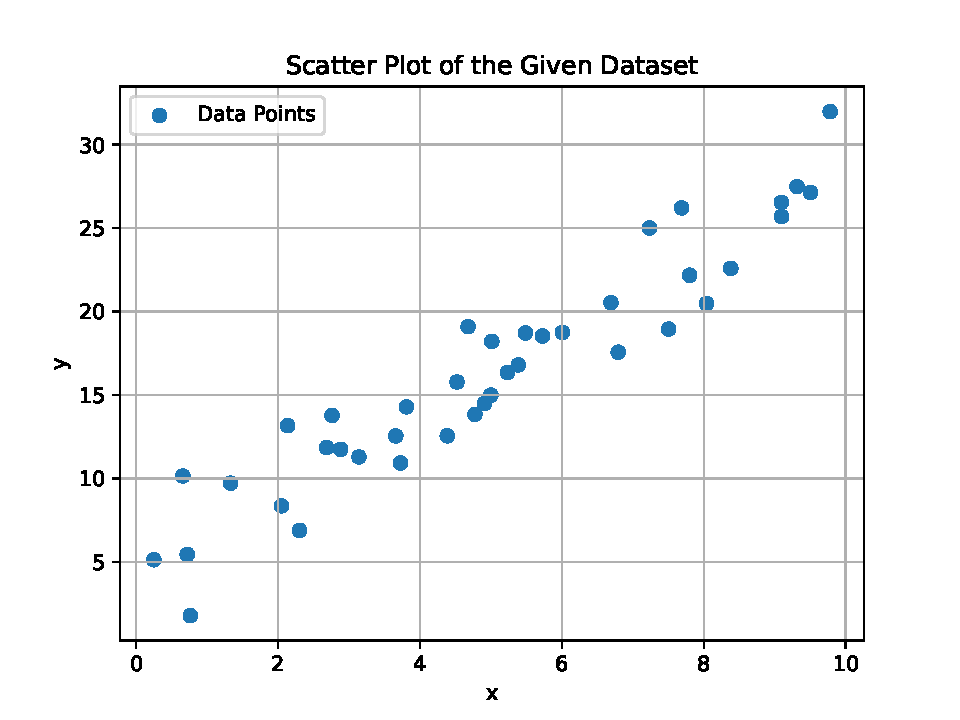
\includegraphics[width=0.85\textwidth]{../q2/Points.pdf}
    \caption{Scatter Plot of the Generated Dataset}
\end{figure}

\subsection{Construction of the Design Matrix}

For a linear model with an intercept and a slope,
the design matrix is constructed as

\begin{equation}
X=
\begin{bmatrix}
1&x_1\\
1&x_2\\
\vdots&\vdots\\
1&x_n
\end{bmatrix}.
\end{equation}

The coefficient vector is

\begin{equation}
\boldsymbol{\beta}=
\begin{bmatrix}
\beta_0\\
\beta_1
\end{bmatrix}.
\end{equation}

The model can therefore be expressed in matrix form as

\begin{equation}
\boxed{y=X\boldsymbol{\beta}+\epsilon}.
\end{equation}

For the generated dataset, the dimensions of
the design matrix are

\begin{equation}
\boxed{\operatorname{shape}(X)=(40,2)}.
\end{equation}

Its rank is

\begin{equation}
\boxed{\operatorname{rank}(X)=2}.
\end{equation}

Since the rank is equal to the number of columns,
the two columns are linearly independent.

\subsubsection{Why Does No Exact Line Pass Through Every Point?}

The generated observations contain random noise.
Consequently, the values of $y$ are not an exact
linear combination of the two columns of $X$.

In other words,

\begin{equation}
y\notin\operatorname{Col}(X).
\end{equation}

Therefore, there is generally no coefficient vector
$\boldsymbol{\beta}$ satisfying

\begin{equation}
X\boldsymbol{\beta}=y
\end{equation}

for every observation.

Instead, the least-squares method finds a vector
in the column space of $X$ that is closest to
the observation vector $y$ in the Euclidean norm.

\subsection{Part B: Solving Using the Normal Equations}

The least-squares problem is to find the coefficient
vector $\boldsymbol{\beta}$ that minimises

\begin{equation}
\|y-X\boldsymbol{\beta}\|^2.
\end{equation}

Expanding the expression gives

\begin{equation}
\begin{aligned}
\|y-X\boldsymbol{\beta}\|^2
&=(y-X\boldsymbol{\beta})^T
(y-X\boldsymbol{\beta})\\
&=y^Ty-2\boldsymbol{\beta}^TX^Ty
+\boldsymbol{\beta}^TX^TX\boldsymbol{\beta}.
\end{aligned}
\end{equation}

Differentiating with respect to $\boldsymbol{\beta}$
and equating the result to zero gives

\begin{equation}
-2X^Ty+2X^TX\boldsymbol{\beta}=0.
\end{equation}

Rearranging,

\begin{equation}
X^TX\boldsymbol{\beta}=X^Ty.
\end{equation}

These equations are known as the normal equations.

Since $X$ has full column rank, $X^TX$ is
invertible. Therefore,

\begin{equation}
\boxed{
\boldsymbol{\beta}
=(X^TX)^{-1}X^Ty
}.
\end{equation}

In the implementation, the system is solved directly
using

\begin{equation}
\texttt{np.linalg.solve(X.T@X,X.T@y)}
\end{equation}

rather than explicitly calculating the inverse.

\subsubsection{Calculated Regression Coefficients}

The computed coefficients are

\begin{equation}
\boxed{\beta_0=4.438044609693186}
\end{equation}

and

\begin{equation}
\boxed{\beta_1=2.389119876178245}.
\end{equation}

The actual coefficients used to generate the data
were

\begin{equation}
\beta_0=4,\qquad \beta_1=2.5.
\end{equation}

The calculated values are not exactly equal to
the original coefficients because random noise
was added to the observations.

The resulting fitted regression equation is

\begin{equation}
\boxed{
\hat{y}
=4.43804461+2.38911988x
}.
\end{equation}

\subsubsection{Comparison with NumPy Least Squares}

The solution is compared with the built-in function

\begin{equation}
\texttt{np.linalg.lstsq(X,y,rcond=None)}.
\end{equation}

The resulting coefficient vector is

\begin{equation}
\begin{bmatrix}
4.43804461\\
2.38911988
\end{bmatrix}.
\end{equation}

The comparison using \texttt{np.allclose}
returns \texttt{True}, confirming that both
methods produce numerically equivalent solutions.

\subsubsection{Fitted Regression Line}

The fitted regression line is plotted along with
the original observations.

\begin{figure}[H]
    \centering
    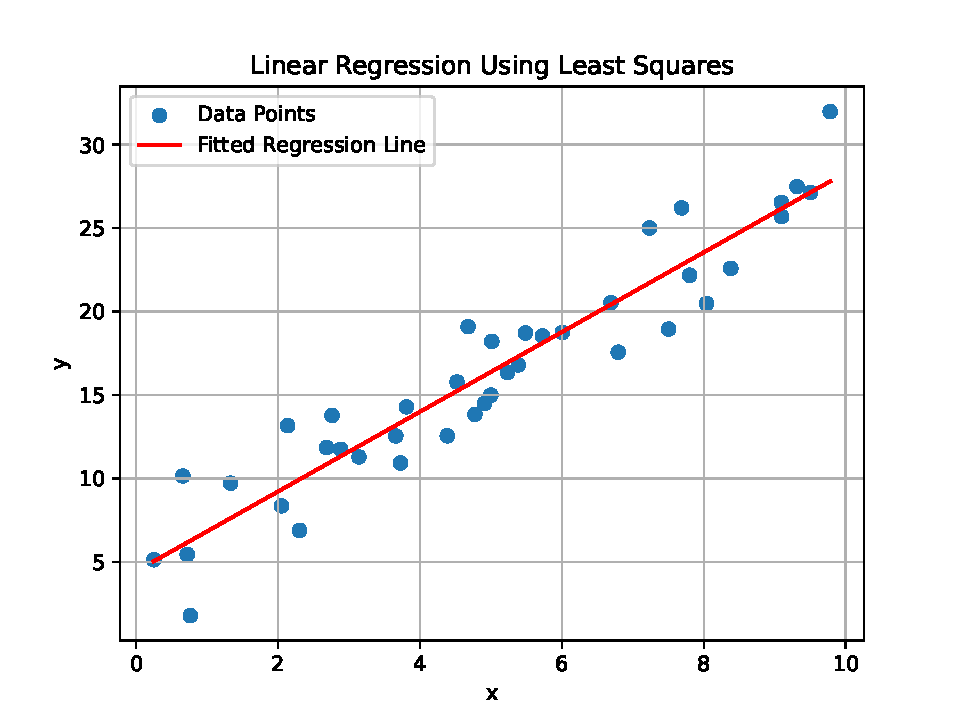
\includegraphics[width=0.85\textwidth]{../q2/Fit-Model.pdf}
    \caption{Generated Dataset with the Fitted Regression Line}
\end{figure}

The fitted line represents the least-squares
approximation of the generated observations.

\subsection{Part C: Geometry of the Least-Squares Fit}

The least-squares solution has an important
geometrical interpretation.

The fitted vector is defined as

\begin{equation}
\boxed{\hat{y}=X\boldsymbol{\beta}}.
\end{equation}

Since it is obtained as a linear combination
of the columns of $X$, the fitted vector
necessarily belongs to the column space of $X$:

\begin{equation}
\hat{y}\in\operatorname{Col}(X).
\end{equation}

The residual vector is defined as

\begin{equation}
\boxed{r=y-\hat{y}}.
\end{equation}

It represents the difference between the original
observation vector and its fitted approximation.

\subsubsection{Orthogonality of the Residuals}

From the normal equations,

\begin{equation}
X^TX\boldsymbol{\beta}=X^Ty.
\end{equation}

Rearranging,

\begin{equation}
X^T(y-X\boldsymbol{\beta})=0.
\end{equation}

Since

\begin{equation}
r=y-X\boldsymbol{\beta},
\end{equation}

we obtain

\begin{equation}
\boxed{X^Tr=0}.
\end{equation}

This condition states that the residual vector
is orthogonal to every column of the design matrix.

The numerical verification gives

\begin{equation}
\texttt{np.allclose(X.T@r,0)}
=\texttt{True}.
\end{equation}

\subsubsection{Sum of the Residuals}

The first column of the design matrix consists
entirely of ones.

Therefore, the first component of $X^Tr=0$ gives

\begin{equation}
\begin{bmatrix}
1&1&\cdots&1
\end{bmatrix}r=0.
\end{equation}

Hence,

\begin{equation}
\boxed{\sum_{i=1}^{n}r_i=0}.
\end{equation}

The computed sum of residuals is

\begin{equation}
9.237055564881302\times10^{-14}.
\end{equation}

This value is approximately zero. The small
difference from exact zero is due to floating-point
rounding in numerical computation.

\subsubsection{Projection Matrix}

The orthogonal projection matrix onto the column
space of $X$ is defined as

\begin{equation}
\boxed{
P=X(X^TX)^{-1}X^T
}.
\end{equation}

Applying this matrix to the observation vector gives

\begin{equation}
Py=X(X^TX)^{-1}X^Ty.
\end{equation}

From the normal equations,

\begin{equation}
(X^TX)^{-1}X^Ty=\boldsymbol{\beta}.
\end{equation}

Therefore,

\begin{equation}
\boxed{Py=X\boldsymbol{\beta}=\hat{y}}.
\end{equation}

The numerical verification confirms

\begin{equation}
\texttt{np.allclose(P@y,y\_cap)}
=\texttt{True}.
\end{equation}

\subsubsection{Idempotence of the Projection Matrix}

A projection matrix must satisfy

\begin{equation}
\boxed{P^2=P}.
\end{equation}

To verify this property,

\begin{equation}
\begin{aligned}
P^2
&=X(X^TX)^{-1}X^T
X(X^TX)^{-1}X^T\\
&=X(X^TX)^{-1}
(X^TX)
(X^TX)^{-1}X^T\\
&=X(X^TX)^{-1}X^T\\
&=P.
\end{aligned}
\end{equation}

Thus, projecting a vector that has already
been projected does not change it.

The numerical verification gives

\begin{equation}
\texttt{np.allclose(P@P,P)}
=\texttt{True}.
\end{equation}

\subsubsection{Trace of the Projection Matrix}

The trace of a square matrix is the sum of
its diagonal elements.

For this projection matrix,

\begin{equation}
\operatorname{trace}(P)=\operatorname{rank}(X).
\end{equation}

Since the design matrix has rank $2$,

\begin{equation}
\boxed{\operatorname{trace}(P)=2}.
\end{equation}

The computed value is

\begin{equation}
\operatorname{trace}(P)=1.999999999999999.
\end{equation}

This is approximately equal to $2$, as expected.

\subsubsection{Pythagorean Theorem}

The fitted vector and residual vector are
perpendicular because

\begin{equation}
\hat{y}^Tr=0.
\end{equation}

Since

\begin{equation}
y=\hat{y}+r,
\end{equation}

taking the squared Euclidean norm gives

\begin{equation}
\begin{aligned}
\|y\|^2
&=(\hat{y}+r)^T
(\hat{y}+r)\\
&=\|\hat{y}\|^2
+2\hat{y}^Tr+\|r\|^2.
\end{aligned}
\end{equation}

The middle term is zero due to orthogonality.
Therefore,

\begin{equation}
\boxed{
\|y\|^2=
\|\hat{y}\|^2+\|r\|^2
}.
\end{equation}

The numerical verification confirms that this
identity holds within floating-point precision.

\subsubsection{Geometrical Interpretation of the Projection}

The least-squares solution can be understood
as an orthogonal projection of the observation
vector $y$ onto the column space of the design
matrix $X$.

The fitted vector

\begin{equation}
\hat{y}=X\boldsymbol{\beta}
\end{equation}

is a linear combination of the columns of $X$.
Therefore, it lies within $\operatorname{Col}(X)$.

The residual

\begin{equation}
r=y-\hat{y}
\end{equation}

represents the difference between the original
observation vector and its fitted approximation.

The condition

\begin{equation}
X^Tr=0
\end{equation}

shows that the residual is perpendicular to
every column of $X$. Since every vector in
the column space is a linear combination of
these columns, the residual is perpendicular
to the entire column space.

Consequently, the fitted vector is the point
in the column space closest to the original
observation vector, measured using the
Euclidean distance. Any other vector in the
column space would produce a residual with
a larger norm.

The projection matrix provides another
verification of this interpretation. The equality

\begin{equation}
Py=\hat{y}
\end{equation}

shows that applying the projection matrix
to $y$ produces the fitted vector.

Its idempotence,

\begin{equation}
P^2=P,
\end{equation}

confirms that applying the projection again
does not change the fitted vector.

Furthermore, the trace of the projection matrix
is approximately $2$, matching the rank of $X$
and hence the dimension of its column space.

Finally, the Pythagorean identity

\begin{equation}
\|y\|^2=
\|\hat{y}\|^2+\|r\|^2
\end{equation}

confirms that the fitted component and residual
component are perpendicular.

Together, these results establish that
$\hat{y}$ is the orthogonal projection
of $y$ onto $\operatorname{Col}(X)$.

\subsection{Part D: Solving Using QR Decomposition}

The least-squares problem can also be solved
using QR decomposition without explicitly
forming the normal equations.

The design matrix is decomposed as

\begin{equation}
X=QR,
\end{equation}

where the columns of $Q$ are orthonormal and
$R$ is upper triangular.

Thus,

\begin{equation}
Q^TQ=I.
\end{equation}

The normal equations are

\begin{equation}
X^TX\boldsymbol{\beta}=X^Ty.
\end{equation}

Substituting $X=QR$ gives

\begin{equation}
(QR)^T(QR)\boldsymbol{\beta}
=(QR)^Ty.
\end{equation}

Using the transpose property,

\begin{equation}
R^TQ^TQR\boldsymbol{\beta}
=R^TQ^Ty.
\end{equation}

Since $Q^TQ=I$,

\begin{equation}
R^TR\boldsymbol{\beta}
=R^TQ^Ty.
\end{equation}

Because $X$ has full column rank, $R$ is
nonsingular. Therefore, $R^T$ is also
nonsingular and can be cancelled from both
sides.

This gives

\begin{equation}
\boxed{R\boldsymbol{\beta}=Q^Ty}.
\end{equation}

The resulting triangular system can be solved
using the back-substitution algorithm implemented
in Question 1.

\subsubsection{QR Solution}

The vector on the right-hand side is calculated as

\begin{equation}
c=Q^Ty.
\end{equation}

The system

\begin{equation}
R\boldsymbol{\beta}=c
\end{equation}

is then solved using back substitution.

The computed coefficient vector is

\begin{equation}
\boxed{
\boldsymbol{\beta}_{QR}
=
\begin{bmatrix}
4.43804461\\
2.38911988
\end{bmatrix}
}.
\end{equation}

This is compared with the solution obtained
using the normal equations:

\begin{equation}
\boldsymbol{\beta}_{QR}
\approx
\boldsymbol{\beta}_{\mathrm{normal}}.
\end{equation}

The numerical comparison using \texttt{np.allclose}
returns \texttt{True}.

Thus, both approaches produce the same
least-squares solution within numerical precision.

\subsection{Conclusion of Question 2}

The generated dataset was successfully modelled
using linear regression.

The normal equations produced the regression
coefficients, and the result was verified against
NumPy's least-squares routine.

The residual orthogonality condition, projection
matrix properties, trace, and Pythagorean identity
confirmed the geometrical interpretation of the
least-squares solution.

Finally, QR decomposition and back substitution
produced the same regression coefficients,
demonstrating an alternative method for solving
the least-squares problem.

\subsection{Source Code Location}

\begin{lstlisting}[frame=single, basicstyle=\ttfamily\small, columns=fullflexible, escapeinside={(*@}{@*)}]
(*@\makebox[\dimexpr\linewidth-2\fboxsep-2\fboxrule\relax][c]{\texttt{\detokenize{../q2/EE26BTECH11230q2.py}}}@*)
\end{lstlisting}

%================================================
% OVERALL CONCLUSION
%================================================

\newpage

\section{Overall Conclusion}

The two questions demonstrate the application
of fundamental concepts in matrix theory and
linear algebra through numerical computation.

The first question implemented Gram--Schmidt
orthogonalisation and QR decomposition. The
orthogonality of the resulting matrix, reconstruction
of the original matrix, projection matrix properties,
and solution of a linear system were successfully
verified.

The second question applied least-squares methods
to a generated dataset. The regression coefficients
were calculated using the normal equations and
verified using NumPy's least-squares routine.
The geometrical properties of the solution were
examined through residual orthogonality and
projection matrices.

The QR decomposition approach provided an
independent method for obtaining the same
least-squares coefficients.

Overall, the numerical results agree with the
theoretical properties of orthogonalisation,
projection, and least-squares approximation.

%================================================
% APPENDIX
%================================================

\newpage

\appendix

\section{Additional Numerical Results}

\subsection{Question 1: Linear System Solution}

The QR solution was

\begin{equation}
x=
\begin{bmatrix}
0\\1\\2
\end{bmatrix}.
\end{equation}

The NumPy solution was

\begin{equation}
x_{\mathrm{NumPy}}=
\begin{bmatrix}
0\\1\\2
\end{bmatrix}.
\end{equation}

The difference between the two solutions was

\begin{equation}
\begin{bmatrix}
0\\0\\0
\end{bmatrix}.
\end{equation}

\subsection{Question 2: Regression Results}

The calculated regression coefficients were

\begin{equation}
\boldsymbol{\beta}=
\begin{bmatrix}
4.438044609693186\\
2.389119876178245
\end{bmatrix}.
\end{equation}

The design matrix had dimensions

\begin{equation}
\operatorname{shape}(X)=(40,2)
\end{equation}

and rank

\begin{equation}
\operatorname{rank}(X)=2.
\end{equation}

The sum of residuals was

\begin{equation}
\sum r_i
=9.237055564881302\times10^{-14}.
\end{equation}

The trace of the projection matrix was

\begin{equation}
\operatorname{trace}(P)=1.999999999999999.
\end{equation}

The numerical checks for residual orthogonality,
projection matrix idempotence, and the Pythagorean
identity all returned \texttt{True}.

The QR solution was

\begin{equation}
\boldsymbol{\beta}_{QR}
=
\begin{bmatrix}
4.43804461\\
2.38911988
\end{bmatrix}.
\end{equation}

It agreed with the solution obtained using
the normal equations.

\end{document}
